% vim:tw=72 sw=2 ft=tex
%         File: MF2043Summary.tex
% Date Created: 2015 Dec 17
%  Last Change: 2015 Dec 21
%     Compiler: make
%       Author: Adam Lang
\documentclass[12pt,a4paper]{article}
\usepackage{amsmath, amssymb}
\usepackage[utf8]{inputenc}
\usepackage[T1]{fontenc}
\usepackage[english]{babel}
\usepackage{graphicx}
\usepackage{circuitikz}
\usepackage{gb4e}

\graphicspath{{pics/}}

\title{Summary MF2043 - Robust Mechatronics}
\author{Adam Lang}

\begin{document}

\maketitle


%-------------------Development models-------------------------



\section{Development models}
  \subsection{V-Model}

The V-Model is used when developing new products. It is a way to model
both hardware and software and is used broadly in the industry.
It has ist name from its v-shape where the horisontal axis represents
time and the vertical axis represents level of abstraction. 

\begin{figure}[!h]
  \centering
  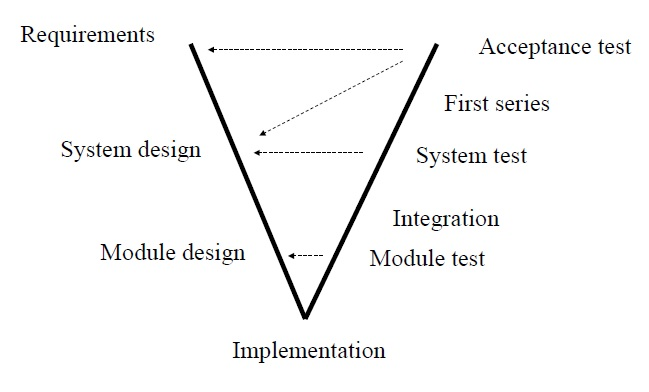
\includegraphics[scale=0.5]{VModel} 
  \caption{Graphical representation of the V-Model}
  \label{fig:Vmodel}
\end{figure}

There are seven different core activities, \textbf{Requrements analasys} 
is the first step and there are collected by analyzing the needs of the 
user(s). It is important to make the requirements measurable so that it
will be fairly easy to see if they have been fulfilled or not. The 
\textbf{system design} is where the engineers analyse the 
buisness of the proposed system from the requirements. 
Their job is to figure out the possibilities and techniques by which the requirements can be
implemented. This is more high level than the next step, \textbf{module
design} this is the lower level design where the system is broken into
smaller units or modules. Each one of them is explained in detail so the
programmer can start coding directly. At the bottom of the V we have the
\textbf{implementation} part where all the parts are implemented and put together
into one system. After the implementation step the testing starts. First
is the \textbf{module tesing} where the individual module is tested.
These are often UTPs (Unit Test Plans) and these are executed to
eliminate bugs at code level. Next is the \textbf{integration testing}
where the coexistance and communicaton of the modules is tested. The
\textbf{system testing} is done to ensure that the expectations of the
customer is met. Once the system testing is complete, ther will be a
\textbf{first series} done. After all this the final test is the
\textbf{user acceptance testing} or UAT. These tests is done in the user
enviroment it is supposed to opperate in.

\subsection{General mechatronic development}

It is important to have the whole system in mind and to look at all
diciplines when developing the system. It is important to have the
software developers develop testing frameworks for the hardware early in
the process and the mechanical designers to have the cabling in mind
when designing the mechanical system. It is also important to see the
specifications as dynamic, they will change during the work process. 


%----------------------OP AMPS-------------------------------


  \section{Operational Amplifier}
    The two \textbf{golden rules} for op amps:
    \begin{enumerate}
      \item The output attempts to do whatever is nessesary to make the
        voltage differance between the input pins zero. (It "looks" at its
        input terminals and swing its output terminal around so that the
        external feedback-network brings the input differential to zero.
      \item The inputs draw no current.
      \end{enumerate}

    \subsection{Inverting}

    \begin{figure}[!h]
      \begin{center}
        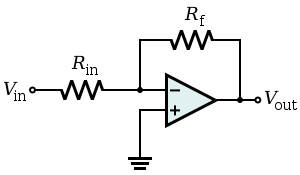
\includegraphics[scale=0.5]{InvOpAmp}
        \caption{The inverting OP-Amp}
        \label{fig:InvOpAmp}
      \end{center}
    \end{figure}
    Let's look at the inverting amp in figure \ref{fig:InvOpAmp}. With the
    golden rules in mind we can see that:
    \begin{enumerate}
    \item The + pin is to ground (might also be to ref) so rule 1
      implies that - also is.
    \item This must mean that the voltage over $R_f$ is $V_{out}$ and
      that the voltage over $R_{in}$ is $V_{in}$.
    \item Using rule 2 we have 
      \begin{equation}
        V_{out}=-\frac{V_{in}R_f}{R_{in}}
      \end{equation}
    \end{enumerate}
    So, how does this work? Let's for simplicity say that
    $R_f=100k\Omega$ and $R_{in}=10k\Omega$ and the input is $+1V$.
    Let's say for the sake of the matter that the output is
    uncooperative and sits at zero. What happens? $R_f$ and $R_{in}$
    form a voltage divider, holding the invertign input at $+0.91V$ The
    op amp sees the enormous inbalance and forces the output to go
    negative. This will continue until the output is at it's requred
    $-10V$. At this point is both the inputs at the same voltage,
    ground. This also means that any tendency to lower the volt lower
    than $-10V$ will pull the inverting input below ground forcing the
    output to rise. The downside with an inverting amplifier is the low
    input impedance
    \\ The - pin can be connected to a reference voltage meaning that it
    will use this as a virtual ground and in so "lifting" the output
    to an offset. This can be used when using a inverting configuration
    for an implementation where the sign invertion is undesired.

    \subsection{Non-Inverting}
    \begin{figure}[!h]
      \begin{center}
        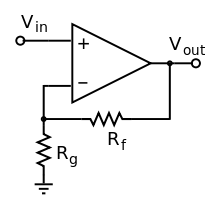
\includegraphics[scale=0.5]{NonInvOpAmp}
        \caption{Non-Inverting Op-Amp}
        \label{fig:NonInvOpAmp}
      \end{center}
    \end{figure}
    The non-inverting operational amplifier as seen in figure 
    \ref{fig:NonInvOpAmp} have the desired infinite input impedance.
    This is almost true for most amps, some, like a JFET 411 input it
    would be $10^12$. The output impedance is however still a fration of
    an ohm.\\
    The simple analisys will give that $V_- = V_{in}$ but $V_-$
    comes from a voltage divider, $V_-=V_{out}/(R_g+R_g)$. Set
    $V_-=V_{in}$ and you will get a gain of
    \begin{equation}
        G_V=1+\frac{R_f}{R_g}
        \label{eq:gainNonInv}
    \end{equation}
    As seen from equation \ref{eq:gainNonInv} the maximum gain of an
    non-inverting amplifier is 1. This makes the non-inverting amplifier
    unsuitable for some applications. 



%-----------------------------------FILTERS--------------------------------


    \section{Filters}
  A filter is a circut or a software that performes signal processing
  functions to remove frequency components from the signal, to enhance
  wanted ones, or both. There are many types of filters some will be
  covered below.
  \subsection{Analog}
  The analoge filter is a filter that will process the analog signal,
  comming straight from the harware. The source will often be a sensor
  of some sort, vibration, sound, temperature, extension etc. 
  \subsubsection{Anti-alias lowpass filter}
  Aliasing is an effect where different signals will become
  indestinguishable when sampled. If a signal with noise is sampled
  there will be no way of differentiatiating the noise from the signal.
  There is a variety of implementations for when a analog signal will 
  be digitilized, audio beeing one of the most intuitive. The convertion
  between analog and digital is done by sampling the amplitude of the
  analog signal and convert each sample to a numeric quantity. This
  process can introduce artefacts, or missleading amplitudes due to both the
  finite accuracy by which the values are quantizied and brought from
  the continuos to the descrete and from the finite rate at which these
  samples are taken. The \textbf{Nyqvist criterion} says that the signal
  beeing digitilized can not contain frequencies that exceeds half the
  sampling rate $f_s$. This is usualy accomplished by passing the signal
  through a \textbf{anti-aliasing filter} whose cutoff frequency $f_c$
  ensures thorough attenuation of signals above the Nyqvist frequency
  $f_s/2$. In short the banwidth of the signal is restricted to satisfy
  the samplin theorem that states that the unambiguous reconstruction of
  the signal from its samples is possible if the power of the
  frequencies over the Nyqvist criterion is zero. In real life it is a
  trade off between bandwidth and aliasing. 
  \begin{exe}
    \ex Example: \\
    You have a signal from a sensor that you are sampling at $f_s = 1kHz$.
    What should be you cutoff frecuency $f_c$? \\
    \textbf{Answer:} $f_c = f_s/2 = 500 Hz$ Due to the Nyqvist criterion.
  \end{exe}
  \subsubsection{Passive filters}
  There are a veriety of different passive filters both high- and low
  pass. The simpelest filters are presented below.
  \begin{figure}[!h]
  \begin{center}
      \begin{circuitikz}[european]
        \draw(0,0)
        node[left]{-}
        to[short, o-] (2,0) 
        to[C, l=$C$, *-*] (2,2)
        to[R, l=$R$, -o] (0,2)
        node[left] {+}
        to[open, o-o] (0,0);
        
        \draw(2,0)
        to[short] (4,0)
        node[right]{-}
        to[open, o-o] (4,2)
        node[right]{+}
        to[short] (2,2);

      \end{circuitikz}
      \caption{Passive RC low pass filter}
      \label{fig:passRC}
    \end{center}
  \end{figure}

  \begin{figure}[!h]
    \begin{center}
      \begin{circuitikz}[european resistors]
        \draw
        (0,0) node[left]{-}
        to[short]
        (2,0) to[L, l=$L$, *-*]
        (2,2) to[R, l=$R$]
        (0,2) node[left]{+}
        to[open, o-o]
        (0,0);
        \draw
        (2,0) to[short]
        (4,0) node[right]{-}
        to[open, o-o]
        (4,2) node[right]{+}
        to[short]
        (2,2);
      \end{circuitikz}
      \caption{Passive RL high pass filter}
      \label{fig:passRL}
    \end{center}
  \end{figure}

  The filters seen in figure \ref{fig:passRC} and figure \ref{fig:passRL} have
  counterparts for when using an RC highpass and a RL lowpass. The
  components will then change place and for the resistor will then
  connect to ground. The way the RC low pass filter works is that at low
  frequencies will the hight reactance offered by the capacitor allow
  almost all of the input signal to develop as an output over the
  capacitors inductance, $X_C$. When the frequenzy increases will R
  become significantly larger than $X_C$. This will make the circuit
  attenuate the the higher frequiencies and send them straight to
  ground. The band of frequencies that the filter will attenuate depends
  on the value for the components. The components relative value of
  $X_C$ and $R$ will determine how the gain, $V_{out}/V_{in}$ is
  different. The gain for a passive filter is always $<1$ due to the out
  impedance beeing too high. The output voltage can be found by using
  \begin{equation}
    V_{out}=\frac{1}{(1+\omega^2R^2C^2)^{1/2}}V_{in}.
  \end{equation}
  The cutoff frequency for a passive filter is found as
  \begin{equation}
    f_c=\frac{1}{2\pi RC}.
  \end{equation}
  The signal driving the filter sees a load
  of R plus the load resistance at low frequencies, dropping to just $R$
  at high frequencies. The worst case source and load impedance of an RC
  filter are both equal to $R$.\\

    \subsubsection{Active Filters}
    Active filters ar mainly to gain the amplitude of the the signal.
    Since a passive filter will result in a voltage drop the active
    filter might be used where the signal needs to be amplified. This
    can be useful if the signal sourse e.g. a sensor, feeds very little
    signal. It us also useful due to the fact that is can feed more
    current than the source can. The active filter is most often built
    of an operational amplifier.\\
    A \textbf{first order active low pass filter} will be a inverting
    amplifier and a capacitor in parallel with $R_2$ as seen in figure 
    \ref{fig:1ordActLowPass}
    \begin{figure}[!h]
      \begin{center}
        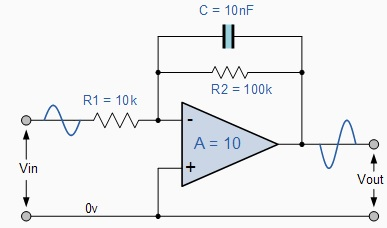
\includegraphics{1ordActLowPass}
        \caption{Inverting first order active low pass filter}
        \label{fig:1ordActLowPass}
      \end{center}
    \end{figure}
    This will have the amplification,
    \begin{equation}
      A_Ninv=-\frac{R_2}{j\omega CR_1R_2+R_1}
    \end{equation}
    and the cutoff frequency,
    \begin{equation}
      f_c=\frac{1}{2\pi R_2C}.
    \end{equation}
    \begin{figure}[!h]
      \begin{center}
        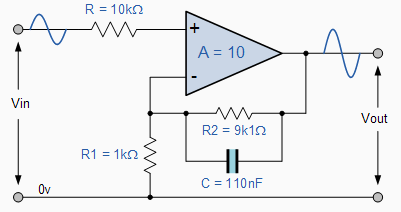
\includegraphics{1ordNonInvActLowPass}
        \caption{Non-Inverting first order low pass filter}
        \label{fig:1ordNonInvLowPass}
      \end{center}
    \end{figure}
    The non-inverting amplifier have the advantage of having a very high
    impedane between the input pins. But the sam problem as previously
    disscussed apply here, the lowest amplification is 1, meaning that
    the amplifier can not be used to damp a signal. There solution will
    also filter quite badly with low amplifications. \\
    A thing to keep in mind when designing active filters is that
    resistors and capacitors must be provided after the set filter
    charataristics.

    \subsubsection{Higher order active low pass filter}
    The Sallen-Key low pass filter is the basis for many of the well
    known filters such as \textbf{Butterworth}, \textbf{Bessel} and
    \textbf{Chebyshev} filters.
    \begin{figure}[!h]
      \begin{center}
        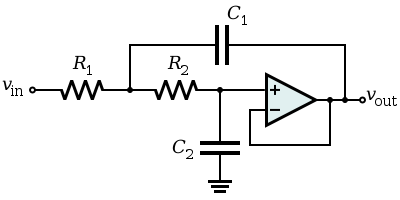
\includegraphics[scale=0.5]{sallenKey}
        \caption{Second order Sallen-Key low pass filter}
        \label{fig:sallenKey}
      \end{center}
    \end{figure}\\
    \textbf{Butterworth} this will give aflat frequency responce in the
    pass band. To design a butterwort filter, all sections
    have the same values of $R$ and $C$ given simply $RC=1/2\pi f_c$\\
    \textbf{Bessel} filters have linear phase or
    constant group delay in the pass band. They are not that more complicated
    than the Butterworth. Within each section we have $R_1=R_2=R$ and
    $C_1=C_2=C$ but the $RC$ products for each section is different and
    must be scales. According to this we therefor have $RC=1/2\pi
    c_nf_c$\\
    \textbf{Chebyshev} have a steep roll off and a ripple in the
    passband or the stopband. They have the same calculations as a
    Bessel filter. \\
    The filters above are in their standar configuration a secon order
    filter. To obtain a higher order filter ju simply multiply the
    Sallen-Key filters, this will give you a even order filter. To
    obtain a odd order filter ypu simply add one extra single order
    filter. 

  \section{Power Supply}
    Due to the vast number of different power sources, ranging from the
    socket in the wall to solar panels and fuel cells. There is a
    obvious need for converters and regulators. The regulators can
    convert AC to DC, DC to DC (regulating) or invert from DC to AC.

    \subsection{Linear Regulator}
    The linear regulator is generaly a linear control element in series
    with the dc input. This is then regulated with a feedback to hace a
    constant output. \\
    The linear regulator is still widely used for its low noise output
    in applications where there is a need for precise output. The
    dissadvantages with the linear regulator is it's low effectiveness
    due to power dissipation in the control element. This will introduce
    the need for heatsink and result in wasted power. The output is
    always lower than the input.


    \subsection{Switching Regulator}
    In the switched regulator, a transistor is operated by a saturared
    switch (oscillator) that periodicly applies the full unregelated voltage across
    an inductor for short intervals. The inductors current builds up
    during each pulse storing $E_L=1/2LI^2$ in it's magnetic field. 
    When the switch is turned off, some or all of the stored energy is
    transferred to a filter capacitor at the output which also smooths
    the output. Like the linear regulator, a feedback compares the
    output with a voltage reference, but it's the ocsillator that
    controls the output by changing the oscilator frequency.
    The switcher is nowadays widely used in all types of electronic
    applications. Since the control element is either off or saturated,
    there is very little power dissipation. This efficiency is good
    since less losses means that the components can be made smaller due
    to the fact that less heat is generated. The downsides is that there
    output is considerably more noisy than the linear regulator due to
    the switching. 
    \subsubsection{Step down (buck) converter}
    The switch is usualy a MOSFET and the diode is used as a rectifier.
    $V_{out}<V_{in}$
    \begin{figure}[!h]
      \begin{center}
        \begin{circuitikz}[european resistors]
          \draw
          (0,0) node[left]{$+V_{in}$}
          to[short, o-]
          (1,0) to[switch]
          (3,0) to[L, l=$Ferrite Core$]
          (5,0) to[short,-o]
          (6,0) node[right]{$+V_{out}$};
          \draw
          (1,-2) node[ground]{}
          to[pC, -*]
          (1,0);
          \draw
          (3,-2) node[ground]{}
          to[sD*, -*]
          (3,0);
          \draw
          (5,-2) node[ground]{}
          to[pC, -*]
          (5,0);
        \end{circuitikz}
        \caption{Buck (step-down) converter}
        \label{fig:buck}
      \end{center}
    \end{figure}
    When the switch is closed, $V_{in}-V_{out}$ is applied across the
    inductor causing a linear increasing current $dI/dt=V/L$ to flow
    through the inductor. When the swich opens, iductor current
    continues to flow i the same direction with the "catch diode" now
    conducting to complete the circuit. The inductor now have a fixed
    voltage $V_{in}-V_{diode}$ across it, causing the current to decrese
    linearly. The output capacitor acts as a smoother of the inevitable
    sawtooth ripple. The larger the output capacitor is, the smaller the
    ripple voltage. To complete the circuit in figure \ref{fig:buck}, a
    feedback loop should be added controlling either the pulse, or the
    repetition rate that compares the output to a reference. The duty
    cycle can be found as,
    \begin{equation}
      D=\frac{V_{out}}{V_{in}}
    \end{equation}
    It will have lower $V_{pp}$ ripple than the boost mode ande can have
    a higher power output, up to kW.

    \subsubsection{Step up (boost) converter}
    The switch is usualy a MOSFET and the diode is used as a rectifier.
    $V_{out}>V_{in}$
    \begin{figure}[!h]
      \begin{center}
        \begin{circuitikz}[european resistors]
          \draw
          (0,0) node[left]{$+V_{in}$}
          to[L, l=$Ferrite Core$, o-]
          (2,0) to[sD*]
          (4,0) to[short, -o]
          (5,0) node[right]{$+V_{out}$};
          \draw
          (2,0) to[switch, *-]
          (2,-2) node[ground]{};
          \draw
          (4,-2) node[ground]{}
          to[pC, -*]
          (4,0);
        \end{circuitikz}
        \caption{Boost (step-up) converter}
        \label{fig:boost}
      \end{center}
    \end{figure}

    The switching regulator can, unlike the linear, produce
    output voltages higher than the input voltage. When the switch is
    conducting, the inductor ramps up. When the switch is turned off,
    the inductor tries to maintain constant current, and the voltage
    rises rapidly. The diod turns on and dumps current into the
    capacitor. The output voltage can therefore be much larger than the
    input voltage. The duty cycle for the boost converter can be found
    as,
    \begin{equation}
        D=1-\frac{V_{in}}{V_{out}}  
    \end {equation}
    The boost mode converter can be used when $P_{out}<150W$. The boost
    mode can be driven in continuous and discontinuous mode, with a
    bigger ripple for the discontinuous one and this is also the most
    common. Continuous can get unstable.

    \subsubsection{Isolated DC-DC converters}
    Transformers and optocouplers provide galvanic isolation but this
    might also be done with a physical barrier on the PCB. This will
    minimize creeping and will work up until the voltage can creep
    through the air with a spark or find a conductive way on the PDB. 
    
    \subsubsection{Buck-Boost}

    \begin{figure}[!h]
      \begin{center}
        \begin{circuitikz}
          \draw
          (0,0) node[left]{$+V_{in}$}
          to[short, o-]
          (1,0) to[switch]
          (3,0) to[L, l=$FerriteCore$]
          (5,0) to[sD*]
          (7,0) to[short, -o]
          (8,0) node[right, -o]{$+V_{out}$};
          \draw
          (1,-2) node[ground]{}
          to[pC, -*]
          (1,0);
          \draw
          (3,-2) node[ground]{}
          to[sD*,-*]
          (3,0);
          \draw
          (5,-2) node[ground]{}
          to[switch, -*]
          (5,0);
          \draw
          (7,-2) node[ground]{}
          to[pC, -*]
          (7,0);
        \end{circuitikz}
        \caption{Non-inverting Boost-Buck converter}
        \label{fig:boostBuck}
      \end{center}
    \end{figure}
    The Buck Boost converter will allow overlap of input and output
    voltage range. This might be particulary usefull in a battery
    powered unit. Say you have two AA batteries starting their life at
    3V and ending it at 1.8V, here is an obvious implementation for the
    buck-boost regulator.

    \subsection{Voltage reference}
    There might be situations where a reference voltage is needed. There
    are a number of applications where a precision reference is needed,
    e.g. A/D or D/A conversion, waveform generators or meters etc. There
    are two styles of voltage references, \textbf{2-terminal} (shunt) and
    \textbf{3-terminal} (series). The two-terminal acts lika a zener
    diode, maintaining a constant voltage drop when current is flowing,
    thus the external cuircuit must maintain a stable operating current.
    The three-terminal reference ($V_{in}$, $V_{out}$ and $GND$) act
    like a linear regulator with internal cuircuitry taking care of
    biasing the internal reference (zenor or something else).
    \subsubsection{Zener diode}
    The zener diode is working much like a regular diode operated in the
    reverse-bias region. And will generally allow significant current if
    it is reverse biased above its breakdown voltage. The reverse bias
    is when the p-n junction is operated in reverse, meaning the voltage
    will basicaly draw the holes in the p-junction (in the p-n junction) further away
    from the junction and in so increasing the width of the depletion
    zone and increasing the voltage barrier. There is some downsides to
    the zener diode, it is very sensitive to temperature fluctuation and
    the voltage tolarance is poor exept with expencive high precition
    zeners. 
    \subsection{Thermal characteristics}
    The regulator is very much in need for temperature awareness.
    $P_{in}-P_{out}$ gives the power consumed by the regulator but this
    does not make it obvious for how to claculate the temperature inside
    the circuit. The temperature also controls the maximum current out,
    the more power the regulator consumes, the less current will come
    out from the regulator. \\
    Heatsinks is widely used to get rid of the increased temperatures in
    the ciurcuts and components. The heatsink might be complemented by a
    fan or some smart construction making the box work with the cimney
    effect. The temperature of a die can be calculated with,
    \begin{equation}
      T_{j(max)}=P_D(R_{\Theta JC}+R_{\Theta CS} +R_{\Theta SA})+T_A,
    \end{equation}
    where $j$ is the die, $JC$ is the junction to case, $CS$ is the case
    to heatsink, $SA$ is the heatsink to ambient and $T_A$ is the
    ambient temperature.

    \subsection{Supply protection}
    The powersupply needs to be protected against high voltages,
    reversed voltage, transients etc. Some regulators have buit in
    protection, and others needs the protection externaly. The
    protection against reversed polarity is not always there, there is a
    famous example of the High-Tech Aurora 9 RC airplane radio
    controller hwo got burnt time after time again. One of the simplest way of
    having a reversed polarity protection is to have a diode or a couple
    of diodes like in figure \ref{fig:revDiode}
    \begin{figure}[!h]
      \begin{center}
        \begin{circuitikz}
            \draw
            (0,0) node[left]{-}
            to[Do, *-]
            (1.5,1.5) node[above]{$\tilde{}$}
            to[Do, *-*]
            (3,0) node[right]{+};
            \draw
            (0,0) to[Do, -*]
            (1.5,-1.5) node[below]{$\tilde{}$}
            to[Do]
            (3,0);
          \end{circuitikz}
          \caption{Reverse polarity protection with diodes}
          \label{fig:revDiode}
        \end{center}
      \end{figure}
      Even though the diode is a great tool, one should not forget that
      the diode will have a 0.7-1V drop over it.

    \section{Capacitors}
      There is a vast variety of capasitors to choose from, here is some
      of them with their typical application. They are typicaly used for
      protection against transients and can reduce noise. 
      \begin{enumerate}
        \item Plastic foil capacitor generally have low cost and
          resistance but will only work in lower frequencies and
          will(exept polypropylene) have stability problems. They are
          typicaly used for decoupling, filters and timing circuits. 
        \item Ceramics are often very stable, they work well in high
          temperatures and over all freequencies but are more
          expensive. They are used in applications like oscillators and
          where demands for high frequency is needed.
        \item Electrolytic capacitor have both wet and dry type. Wet are
          used for high C and V but have a high ESR (Equivalent series
          resistance) and the electrolyte eveporate, causing them to
          age. The wet type are typicaly used in power supplies.
          The dry type age well, have lower ESR and are smaller in size.
          Since they are used with high voltage they can cause fire, and
          send backwards voltage, less with higher teperatures. 
        \item Tantalum electrolyte ($\mu F$ or $pF$)
      \end{enumerate}


\end{document}
